\documentclass[t]{beamer}
\usefonttheme[onlymath]{serif}
\usepackage{datetime}
\usepackage[utf8]{inputenc}
\usepackage[T1]{fontenc}
\usepackage{lmodern}
\usepackage[english]{babel}
%\frenchbsetup{CompactItemize=false}


% \usepackage[babel]{csquotes}
% \usepackage[url=false, doi=false, style=science, backend=bibtex, bibencoding=ascii]{biblatex}
% \bibliography{IEEEabrv,bib/OAM}

  
\graphicspath{{img/}}


\mode<presentation> {
	% \useoutertheme{infolines} % Pour les thèmes qui n'ont pas de pied-de-page
	\usetheme{ulaval}
	%\usecolortheme{ulaval}
	% \setbeamercovered{transparent}
	\setbeamercovered{invisible}
	%\setbeamertemplate{navigation symbols}{} % Enlever les icônes de navigation
}


%\usepackage{bm} 
% For typesetting bold math (not \mathbold)
%\includeonlyframes{}

%\usepackage{pgfpages}
%\setbeameroption{show notes on second screen}
%\setbeameroption{show notes}
%\setbeamertemplate{note page}[plain]

\logo{%\includegraphics[height=0.6cm]{COPL}\hspace{.5cm}%
	\includegraphics[height=0.5cm]{UL_P}\hspace{.2cm}\vspace{.85\paperheight}}


\title[Live Textual Data for Risk Selection]{Risk selection using live textual data from the web for commercial underwriting}
%\subtitle[]{}

\author[J-T Baillargeon]{Jean-Thomas Baillargeon, FSA, CERA}
\institute[Laval University] 
{
	École d'actuariat \\
	Laval University, Québec, Canada \\
	\medskip
	{\emph{jean-thomas.baillargeon.1@ulaval.ca}}
}
\newdate{presentation-date}{09}{08}{2018}
\date{\displaydate{presentation-date}} % \today will show current date. 
% Alternatively, you can specify a date.


\AtBeginSection[]{
  \begin{frame}
	\Huge \centerline{\insertsection}
%  \small \tableofcontents[currentsection, hideothersubsections]
  \end{frame} 
}

\begin{document}



\begin{frame}[label=titre, plain]
	\titlepage
	\begin{center}%\includegraphics[height=1.2cWm]{COPL}%
		%\hspace{2cm}
		\includegraphics[height=2cm]{UL_P}\end{center}
\end{frame}



\begin{frame}[label=intro]{Introduction}
	\textbf{Computer and Actuarial Sciences Project}
	\begin{itemize}
		
		\item Natural Language Processing (NLP)
		\item Software Engeneering
		\item Risk classification
		
	\end{itemize}
	
	\textbf{The details of the project}
	\begin{itemize}
		\item Risk Selection
		\begin{itemize}
			\item Support decision making
		\end{itemize}			
		\item Live textual data from the web
		\begin{itemize}
			\item Data gathered live during underwriting
		\end{itemize}
		\item Commercial underwriting
		\begin{itemize}
			\item Limited scope
		\end{itemize}
	\end{itemize}
	
\end{frame}



\begin{frame}[label=intro]{Introduction}
	\textbf{What we tried to do}
	\begin{itemize}
		\item Download unstructured data from Yellow Pages and Google Places
		\item In order to determine a company's activity
		\item While the company is askings for an insurance coverage
	\end{itemize}
\end{frame}


\begin{frame}[label=metho]{Methodology}
	\textbf{Project Pipeline}
	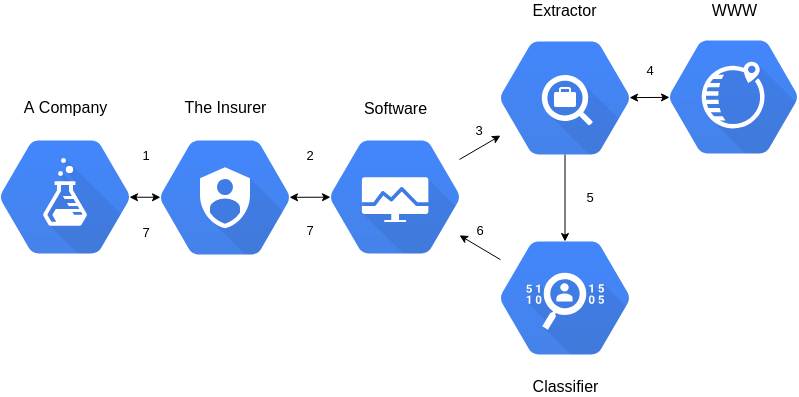
\includegraphics[width=\textwidth]{images/project_pipeline.png}
\end{frame}


\begin{frame}[label=metho]{Methodology}
	\textbf{The Extractor}
	\begin{itemize}
		\item Lot of work
		\item No Universal extractor
		\item Multistep extraction process
	\end{itemize}
\end{frame}


\begin{frame}[label=metho]{Methodology}
	\textbf{Extraction Example}
	
\end{frame}



\begin{frame}[label=metho]{Methodology}
	\textbf{Automating Extraction}
	\begin{itemize}
		\item Crawler and Scrapers
		\begin{itemize}
			\item Mimics the user by browsing without browser
			\item Limitations: user interface design and capcha
		\end{itemize}		
		\item Application Programming Interface (API)
		\begin{itemize}
			\item Communication contract
			\item Controlled acces point to the data\\
			\item Limitations: might not be free
		\end{itemize}	
		\item Extraction Software should support both methods of extraction
	\end{itemize}	
	
\end{frame}



\begin{frame}[label=metho]{Methodology}
	\textbf{Using Textual Data}
	\begin{itemize}
		\item Linking key words to categories 
		\item Using the classifier
	\end{itemize}	
	
	\textbf{Classifier}
	\begin{itemize}
		\item Machine learning algorithm trained to predict class based on words
	\end{itemize}	
	
\end{frame}


\begin{frame}[label=metho]{Methodology}
	\textbf{Training an algorithm}
	\begin{itemize}
			\item Fitting a model or calibration
		\begin{itemize}
		\item \textit{Train} linear regression to predict a value using a vector of numeric variables
		\item \textit{Learn} the $\beta$ that minimize the Mean Square Error in Linear regression
			\end{itemize}	
		\item Classification and regression are supervised learning tasks
		\item Requires a set of $N$ examples with their good answer
		\item Calibrate itself to minimize loss function
	\end{itemize}	
	
\end{frame}


\begin{frame}[label=metho]{Methodology}
	\textbf{Building a Training Data Set}
	\begin{itemize}
		\item Need to create a dataset 
		\begin{itemize}
			\item Linking a company occupancy code, as defined by a classification scheme
			\item To keywords extracted from a source
		\end{itemize}	
		\item The dataset is source specific
		\item Small to medium data
	
	\end{itemize}	
\end{frame}


\begin{frame}[label=metho]{Methodology}
	\textbf{Not Using Big Data in Machine Learning}
	\begin{itemize}
		\item Very different, yet linked concept
		\item Machine Learning is the concept of training algoritmm for specific task
		\item Big Data refers to Data with usage problem due to the 4Vs
		\begin{itemize}
			\item However, certain machine learning algorithms, apt to use big data, became incresingly efficient with the amount of data processed.
		\end{itemize}	
	\end{itemize}
\end{frame}


\begin{frame}[label=metho]{Methodology}
	\textbf{Data Set of Words}
	\begin{itemize}
		\item Not directly usable by machine learning algorithms
		\item NLP solves this problem
		\item Text mining software presented in \cite{francis2010text} implements NLP findings
		\item Change a few blocs beneath the hood
		\item NLP Classification Pipeline
		\begin{itemize}
			\item Tokenization
			\item Transformation
			\item Classification
		\end{itemize}	
	\end{itemize}
\end{frame}


\begin{frame}[label=metho]{Methodology}
	\textbf{Tokenization}
	\begin{itemize}
		\item Split each document $d_i, i \in(1, N)$ into tokens $w_j, j \in (1, M) $ 
		\item In its most basic form, tokens generated $w_j$ are words
		\item Creates a term occurence matrix $S, N \times M$ with elements
		$$ s_{i,j} = 1 \textrm{ if } w_j \in d_i, 0 \textrm{ otherwise}$$
	\end{itemize}
\end{frame}



\begin{frame}[label=metho]{Methodology}
	\textbf{Term Occurence Matrix Example}
	
	
	\begin{table}[H]
		\centering
		\begin{tabular}{|c|c|c|c|c|c|}
			\hline 
			&  broker  & for & hamburger & ... & zebra   \\ 
			\hline 
			Document 1 &    1 & 1 & 0 & ... & 0  \\ 
			\hline 
			Document 2&    0 & 1 & 1 & ... & 1 \\ 
			\hline 
			Document 3 &    0 & 1 & 0 & ... & 1  \\ 
			\hline 
			
		\end{tabular} 
		
	\end{table}
	
\end{frame}


\begin{frame}[label=metho]{Methodology}
	\textbf{Transformation Step}
	\begin{itemize}
		\item Adjust weight for word relevance in the current task
		\item Classification task wants to maximize discrimination between $k$ classes.
		\item Add weight to tokens that are useful
		\item Remove weight to tokens that are useless
		
	\end{itemize}
\end{frame}



\begin{frame}[label=metho]{Methodology}
	\textbf{Matrix Transformation Example}
	
	
	\begin{table}[H]
		\centering
		\begin{tabular}{|c|c|c|c|c|c|}
			\hline 
			&  broker  & for & hamburger & ... & zebra   \\ 
			\hline 
			Document 1 &    1\textbf{(+)} & 1\textbf{(- -)} & 0 & ... & 0  \\ 
			\hline 
			Document 2&    0 &  1 \textbf{(- -)}& 1 \textbf{(+)} & ... & 1\textbf{(-)} \\ 
			\hline 
			Document 3 &    0 & 1 \textbf{(- -)} & 0 & ... & 1\textbf{(-)}  \\ 
			\hline 
			
		\end{tabular} 
		
	\end{table}
	
\begin{itemize}
	\item Metrics for usefulness
	\begin{itemize}
		\item Term Frequency - Inverse Document Frequency (TF-IDF) \cite{Francis2006}, \cite{jurafsky2009speech}
		\item Bi-Normal Separation (BNS)
	\end{itemize}
\end{itemize}

\end{frame}

\begin{frame}[label=metho]{Methodology}
	\textbf{Term Frequency - Inverse Document Frequency (TF-IDF)}
	\begin{itemize}
		\item Intuition
		\begin{itemize}
			\item Useless Word that do not carry meaning would appear in any document, regardless the category
			\item Useful domain related word should occur often in a document
		\end{itemize}
		\item Formula
\end{itemize}
$$ \textrm{tf-idf} = tf(w_i,d_j) \cdot idf(w_i, D)$$
$$tf(i, j) = 0.5 + 0.5 \times \frac{\textrm{count}(w_i, d_j)}{|d_j|}  $$
$$idf(i, D) = \log \frac{|D|}{|\{d \in D :  w_i \in d \}|}$$

\end{frame}


\begin{frame}[label=metho]{Methodology}
	\textbf{Bi-Normal Separation (BNS)}
	\begin{itemize}
				\item Presented in \cite{Forman}
		\item Intuition
		\begin{itemize}
			\item Words that occurs only in documents of a single category are useful
			\item Words occuring randomly in documents are useless
		\end{itemize}
	\end{itemize}
		\begin{table}[H]
		\begin{tabular}{|c|c|c|c|c|c|c|}
			\hline 
			& $C_k$&  broker  & for & hamburger & ... & zebra   \\ 
			\hline 
			Document 1 &  Insurance &  1 (+) & 1(- -) & 0 & ... & 0 \\ 
			\hline 
			Document 2& Zoo &   0 &  1 (- -) & 1 (+) & ... & 1\textbf{(+)} \\ 
			\hline 
			Document 3 & Zoo &  0 & 1 (- -) & 0 & ... & 1\textbf{(+)}  \\ 
			\hline 
			
		\end{tabular} 
		
	\end{table}
\begin{itemize}
		\item Formula
\end{itemize}
$$BNS = abs(\Phi^{-1}(TPR(w_i, D))- \Phi^{-1}(TNR(w_i, D)))$$

\end{frame}


\begin{frame}[label=metho]{Methodology}

	\textbf{True Positive Rate (TPR), False Positive Rate (FPR)}
	\begin{itemize}
		\item Example: 10 documents of known but hidden category, 2 cagories.
		\item Guess class $C_1$ for document $d_i, i = 1,...,N$ if $w_1$ is present.	
\end{itemize}

			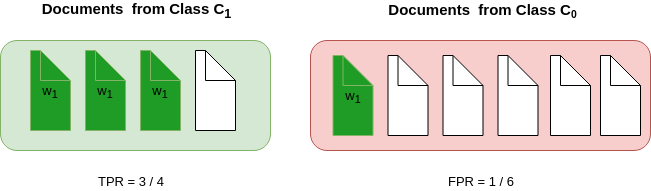
\includegraphics[width=\textwidth]{images/TPRFPR_example.png}

	\begin{itemize}
		
			\item Amongs the guessed docuement:
		\begin{itemize}

			\item \textbf{TPR} = $\frac{\textrm{Number of documents that really belong to } C_1}{\textrm{Total number of documents belonging to } C_1} $
			\item \textbf{FPR} = $\frac{\textrm{Number of documents that do not belong to } C_1}{\textrm{Total number of documents not belonging to } C_1} $
		\end{itemize}
	\end{itemize}

			


\end{frame}

\begin{frame}[label=metho]{Methodology}
		\begin{itemize}
		\item Given TPR = $\frac{3}{4}$ and FPR = $\frac{1}{6}$
			\begin{itemize}
				\item Very useful word
				\item $\textrm{abs}(\Phi^{-1}(\frac{3}{4}) - \Phi^{-1}(\frac{1}{6}) ) = 1.64$ 
			\end{itemize}
		\item Given TPR = $\frac{1}{2}$  and FPR = $\frac{1}{2}$
		\begin{itemize}
			\item Very useless word
			\item $\textrm{abs}(\Phi^{-1}(\frac{1}{2}) - \Phi^{-1}(\frac{1}{2}) ) = 0$ 
		\end{itemize}
	
	\end{itemize}
\end{frame}

\begin{frame}[label=metho]{Methodology}
	\textbf{Bi-Normal Separation}
	\begin{itemize}
		\item Limited to 2 classes (binary classification)
		\item Generalized to $n \geq 2$ classes in this project
	\end{itemize}
\end{frame}


\begin{frame}[label=metho]{Methodology}
	\textbf{Classification Step}
	\begin{itemize}
		\item The actual machine learning algorithm
		\item Prior steps are mandatory preprocessing
		\item Data in matricial form $\boldmath{X}, \boldmath{Y}$ 
		\item Algorithms for classification
		\begin{itemize}
			\item Naive Bayes Classifier, Logistic Regression
			\item Support Vector Machine (SVM), Deep Neural Network (DL)
		\end{itemize}
	\end{itemize}
\end{frame}


\begin{frame}[label=metho]{Methodology}
	\textbf{Naive Bayes Classifier}
	\begin{itemize}
		\item Strong Hypothesis
		\item Very useful baseline algorithm
		\item Given the class of the document, all features are independant
		\item Prediction formula
		$$\hat{y} = \arg\max P(C_k) \prod_{i=1}^{N}p(x_i|C_k)$$
		\item Where \textit{a posteriori} probabilities have been \textit{learned} using the maximum likelyhood estimators.
		
	\end{itemize}
	
	
	
\end{frame}




\begin{frame}[label=metho]{Methodology}
	\textbf{Logistic Classifier}
	\begin{itemize}
		\item A stronger prediction algorithm, 
		\item Liberalized formula \cite{hastie2013elements}
		\item Prediction formula
$$ \hat{y} = \arg\max \beta_{K0} + \boldsymbol{\beta_{K}^T} \cdot  \boldsymbol{x} , $$
		\item Where the parameters have been learned by maximizing the likelihood score

	$$  l(\beta) = \sum_{i=1}^{N} y_i \beta^T x_i - \log(1+ e^{\beta^T x_i}) $$
		
	\end{itemize}
\end{frame}

\begin{frame}[label=metho]{Methodology}
	\textbf{SVM and DL}
	\begin{itemize}
		\item Surprise, no usage in this project
		\item More a proof of concept than an optimal implementation
		\item Black box approach and little room for diagnosis
		\item Questionable appropriateness
	\end{itemize}
\end{frame}


\begin{frame}[label=metho]{Methodology}
	\textbf{Choosing Between Many Categories}
	\begin{itemize}
		\item The classification scheme has $K \geq 200$ classes.
	\end{itemize}

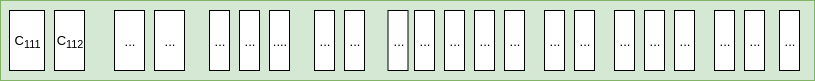
\includegraphics[width=\textwidth]{images/bottom_level.png}
	
	\begin{itemize}
	\item Example of classification
\begin{itemize}
	\item Restaurant - Not Full Licence - Fastfood
	\item Restaurant - Full Licence - Steakhouse
	\item Service - Finance - Accounting
\end{itemize}
\end{itemize}



\end{frame}


\begin{frame}[label=metho]{Methodology}
	\textbf{Choosing Between Many Categories}
	\begin{itemize}
		\item Multiple level classification scheme 
	\end{itemize}
	
	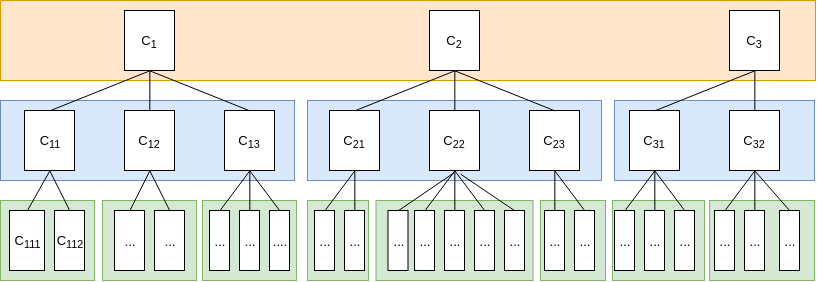
\includegraphics[width=\textwidth]{images/hierarchical_classification.png}
	

\end{frame}


\begin{frame}[label=metho]{Methodology}
	\textbf{Specializing Every Node}
	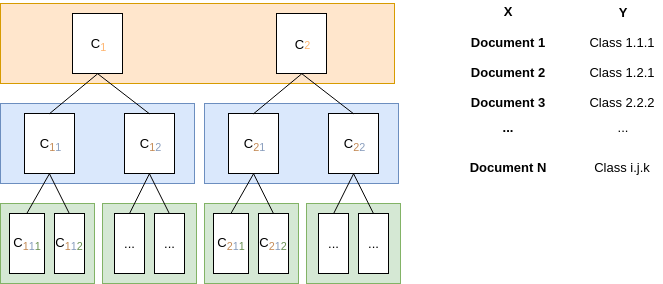
\includegraphics[width=\textwidth]{images/distribution_0.png}
\end{frame}


\begin{frame}[label=metho]{Methodology}
	\textbf{Specializing Every Node}
	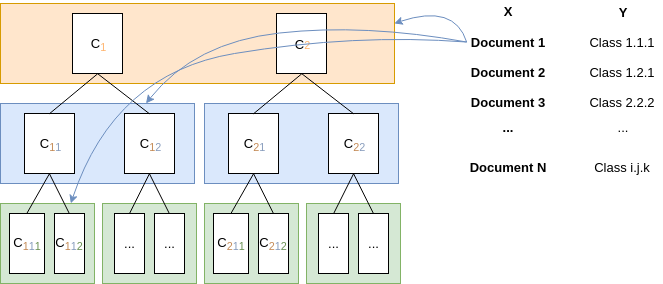
\includegraphics[width=\textwidth]{images/distribution_1.png}
\end{frame}

\begin{frame}[label=metho]{Methodology}
	\textbf{Specializing Every Node}
	
	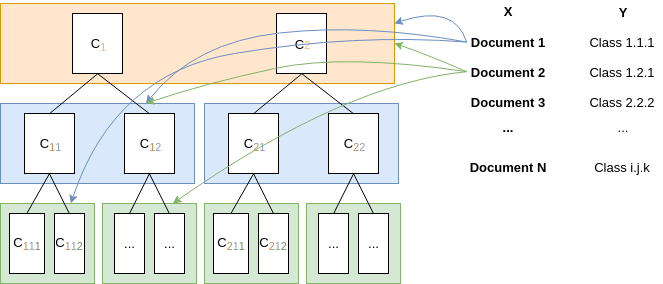
\includegraphics[width=\textwidth]{images/distribution_2.png}
	
	
\end{frame}


\begin{frame}[label=metho]{Methodology}
	\textbf{Specializing Every Node}
	
	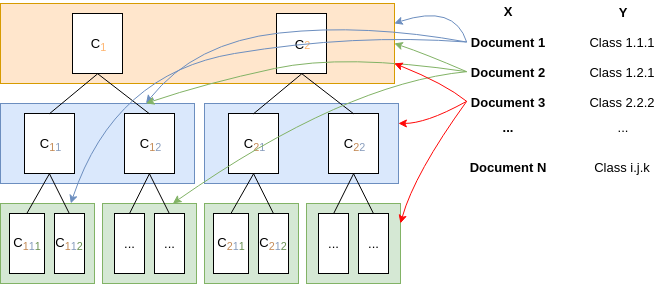
\includegraphics[width=\textwidth]{images/distribution_3.png}
	
\end{frame}


\begin{frame}[label=metho]{Methodology}
	\textbf{Wrap Up}
	
	\begin{itemize}
		\item Build a data set by extracting live data
		\item Train a multi layer hierarchical classifier
	\end{itemize}
	
\end{frame}




\begin{frame}[label=exp]{Experimentation}
	\textbf{And then}
	
	\begin{itemize}
	\item Evaluate the accuracy of the prediction algorithm.
	\item Replicate the calling process, by:
		\begin{itemize}
			\item Holding back one data point
			\item Training the system with $N-1$ data points
			\item Predicting the holded back data Point Occupancy Code
			\item Cycling through all data points, to get average prediction accuracy
		\end{itemize}
	\item Use accuracy evaluation to compare
		\begin{itemize}
			\item Traditional NLP metrics and a dummy classifier 
			\item Traditional NLP metrics and the improvements from this project's work
		\end{itemize}
	\end{itemize}
	
\end{frame}

\begin{frame}[label=exp]{Experimentation}
	\textbf{Data Source Used}
	
	\begin{itemize}
		\item Data from Yellow Pages
		\item Graduately gather over a 10 day period
		\item Counting 1593 data points
	\end{itemize}
	
\end{frame}



\begin{frame}[label=exp]{Experimentation}
	\textbf{Evaluating the Dummy Classifier Performance}
	
	\begin{itemize}
		\item Define the dummy classifier 
		\begin{itemize}
			\item Classifier that would always select the majoritary class
			\item Accuracy = 15\%
		\end{itemize}
		
	\end{itemize}
	
\end{frame}

\begin{frame}[label=exp]{Experimentation}
	\textbf{Traditional NLP Methodology Accuracy}
	
	-	graph 1
	
	-	conclusion
	
\end{frame}




\begin{frame}[label=exp]{Experimentation}
	\textbf{Traditional NLP vs New technique}
	
	-	graph 2
	
	-	conclusion
	
\end{frame}





\begin{frame}[label=conclusion]{Conclusion}
	\textbf{Positive Outcome}
	
	\begin{itemize}
	\item BNS seems to enhance the classification performance
	\item Hierarchical classifier can easily be used to predict higher level class until a significance threshold
	\item Not yet accurate enough for production
	\begin{itemize}
		\item Relatively limited dataset
		\item No efforts to tweek the performance of the algorithm
	\end{itemize}
\end{itemize}
		
	\textbf{Future Work}
	
	\begin{itemize}
		
		\item Get more data / Better coverage for all classes
		\item Combining sources of data
		\item Extend Classification Framework to select optimal node parameters
		
	\end{itemize}
	
\end{frame}


\begin{frame}[label=conclusion]{Conclusion}
\vfill
\begin{centering}
\large\textbf{Questions?}\\

\end{centering}
\end{frame}


\bibliographystyle{apalike2}
\bibliography{ref}

% End of slides
\end{document}